\section{User Interface}\label{sec:design_ui}

In this section we will cover the development of the user interface (UI). First we will cover the requirements and the task that the UI is responsible for solving. Then we will discuss solution approaches for the UI in consideration of our potential users, before finally covering the implementation. 

As a mean to derive requirements, we initially developed an information flow diagram of the UI. This outlined the usage of the system allowing us to consider the different use cases and user needs.

\subsection{Information Flow}

\begin{figure}[tbp]
\centering
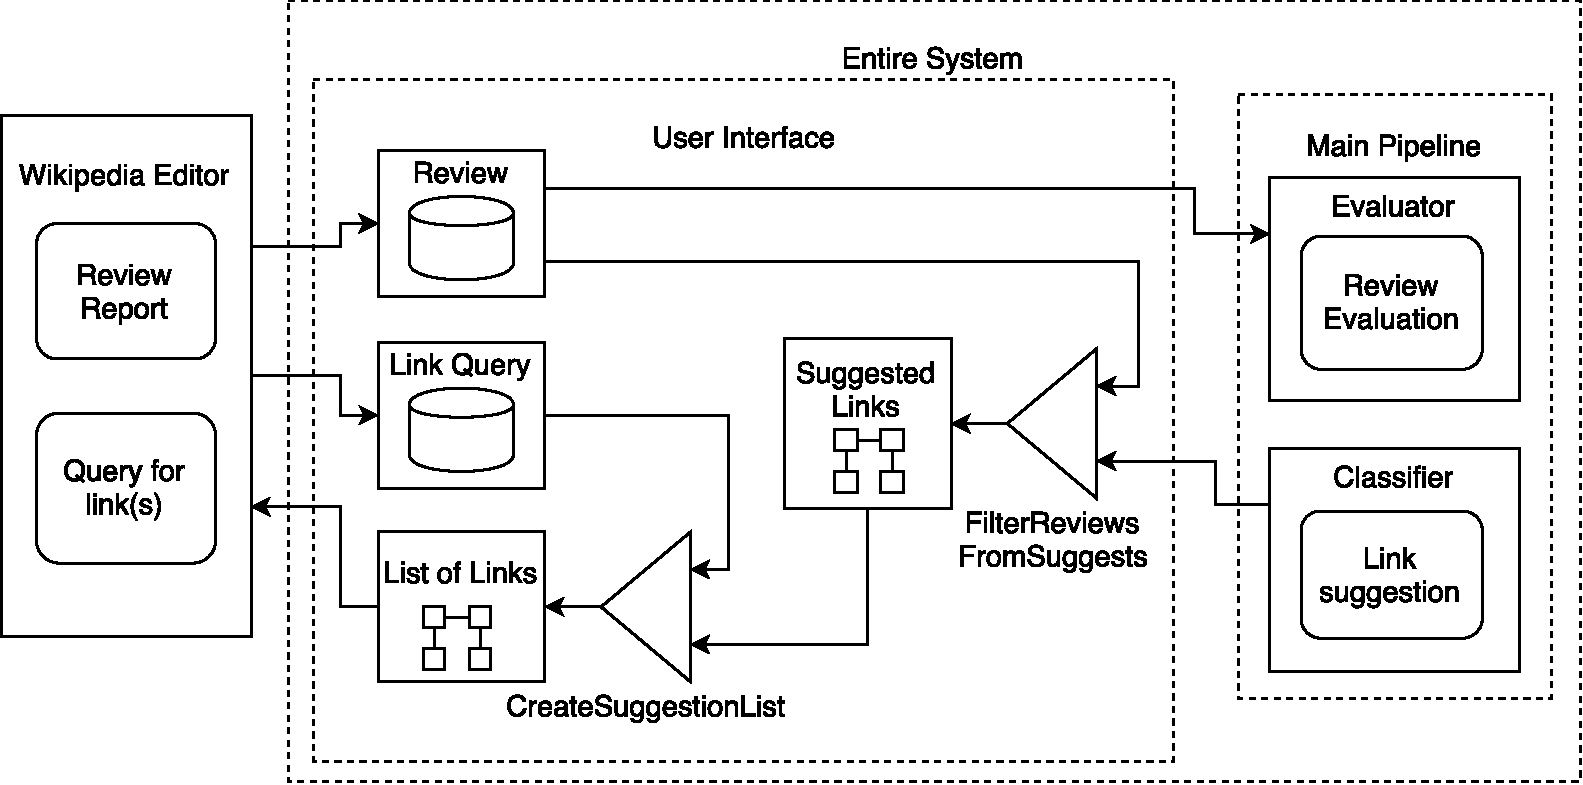
\includegraphics[width=0.95\textwidth]{wikiAPI.pdf}
\caption{Information flow diagram for user interface.}\label{fig:information_flow_UI}
\end{figure}

In the diagram seen in \cref{fig:information_flow_UI}, which is in the WebML+ style~\cite{Casteleyn2009}, we have the two actors and the UI\@. One actor is the Wikipedia Editor and the other is the main pipeline. While the main pipeline could be modeled as a system with its own information flow, it is more beneficial for the requirement engineering process to simplify the main pipeline as an actor outside of the UI, since the requirements for the UI should not be affected by the inner workings of the main pipeline.

The Wikipedia Editor actor has two actions. First is the \enquote{Query for Link(s)} action, which prompts the UI for links to be evaluated. Secondly we have a \enquote{Review Report} action, where the actor informs the UI whether a previously suggested link was added to Wikipedia or not.

While other actions by the Wikipedia Editor actor could easily be conceived, we will argue that these two represent the primary actions, with the \enquote{Query for Link(s)} action being the essential one. By only including these two, we keep the initial requirement analysis focused on the core requirements, and leave further expansion for later iterations.


\subsection{Requirements}

From this diagram two functional requirements can be deducted. There is a requirement for retrieval of link suggestions and a requirement for the reporting of link reviews.

In the case of the retrieval of link suggestions the information flow is as follows:

\begin{enumerate}
	\item The classifier supplies the UI with link suggestions
	\item The reviewed links are filtered from the link suggestions
	\item A Wikipedia Editor queries the UI for links
	\item The query is used to create a list of links for the Editor
\end{enumerate}

For the case of reporting link reviews, where a user reports their evaluation of a suggested link, the information flow is as follows:

\begin{enumerate}
	\item The users submits a report of a suggested link
	\item The review is used for filtering link suggestions
	\item The review is also forwarded to the main pipeline for further evalution
\end{enumerate}

The last step of forwarding the review to the main pipeline represents a future use of the reviews to re-train the classifier. This is not a current consideration in the main pipeline, but the UI is designed to support this type of feedback.

The requirements found in these two information flows are:

\begin{itemize}
	\item A user must be able to query the UI for link suggestions
	\item A user should be able to submit reviews of link suggestion
\end{itemize}

\subsection{Solution Idea}




\subsection{RESTful Web API}